{
\color{red}
\noindent
This chapter should describe the project context, and motivate each of
the proposed aims and objectives.  Ideally, it is written at a fairly
high-level, and easily understood by a reader who is technically
competent but not an expert in the topic itself.

In short, the goal is to answer three questions for the reader.  First,
what is the project topic, or problem being investigated?  Second, why
is the topic important, or rather why should the reader care about it?
For example, why there is a need for this project (e.g., lack of similar
software or deficiency in existing software), who will benefit from the
project and in what way (e.g., end-users, or software developers) what
work does the project build on and why is the selected approach either
important and/or interesting (e.g., fills a gap in literature, applies
results from another field to a new problem).  Finally, what are the
central challenges involved and why are they significant?

The chapter should conclude with a concise bullet point list that
summarises the aims and objectives.  For example:

\begin{quote}
\noindent
The high-level objective of this project is to reduce the performance
gap between hardware and software implementations of modular arithmetic.
More specifically, the concrete aims are:

\begin{enumerate}
\item Research and survey literature on public-key cryptography and
      identify the state of the art in exponentiation algorithms.
\item Improve the state of the art algorithm so that it can be used
      in an effective and flexible way on constrained devices.
\item Implement a framework for describing exponentiation algorithms
      and populate it with suitable examples from the literature on
      an ARM7 platform.
\item Use the framework to perform a study of algorithm performance
      in terms of time and space, and show the proposed improvements
      are worthwhile.
\end{enumerate}
\end{quote}
}

\todo Improve this chapter; not so much technical get a good motivaiton for the study
that doesn't require knowledge about GAs, refer forward in the document

\todo Change genetic algorithm represention to a reference to later chapters

\todo Improve the flow of this paragraph, really lead the reader by the hand,
what are "random means" etc.

Unlike conventional hardware design which relies on experts miticulously creating
specfications, evolvable hardware (EHW) applies genetic algorithms to
flexible hardware platforms to explore the design space of potential
circuit solutions to specified hardware problems \cite{541893}.
The search space of hardware designs is inherrently problematic to maneuver and
genetic algorithms currently have the best track record.
Traversing the set of solutions is of immense difficulty; the fitness landscape
is discontinuous and
search by random means often proves the most fruitful. By combining
the robust nondeterminism inherent in genetic algorithms, and hardware design
one can autonomously develop application specific hardware.

\todo Tell the reader what they are about to read section 1 etc.

\section{Evolvable Hardware}
Decades of evolvable hardware research has explored the application of genetic algorithms to
the domain of hardware design. Genetic algorithms come from the field of natural
computing and use Darwinian-inspired probabilistic procedure to improve a population
of bitstrings'
performance given a fitness criteria with evolutionary pressure \cite{Goldberg:1989:GAS:534133}.
In the case of evolvable hardware,
each individual bitstring can be mapped onto a circuit design
and the fitness critera is rooted
in the circuit's ability to perform some predefined function.

The most common evolvable hardware arrangements
are built on Field Programmable Gate Arrays (FPGAs), these are immensely
flexible integrated circuits and constitute the substrate that the genetic
algorithm creates a solution within. Each member of the population
represents an FPGA configuration, and the fitness is based on the
physical performance of the chip.

Conventional circuit design requires a huge amount of domain specific knowledge.
Applying machine learning to hardware design constitutes a potential
offloading of this information, allowing a user to define the success
criteria for a circuit and letting the machine automously construct a novel solution.
Thus far there have been great successes deploying evolvable hardware to
create user-specific prosthetic hand controllers \cite{Kajitani1999AnEH},
image filters \cite{HybridFilter}, creating arbitrary logic circuits
\cite{Vasicek2011}, and even industrial robot controllers capable of fault recovery \cite{10.1007/3-540-61093-6_6}.
Current solutions are severly limited by scaling issues.

\todo expand on above scaling issues point, talk a lot more about the issues

One of the advantages of genetic algorithms is also one of their largest
weaknesses; they excel in generating strange and esoteric solutions,
which can often outperform their more conventional hand-designed counterparts.
An example of which (although outside the domain of circuit synthesis)
comes from NASA, where an evolutionary algorithm designed an, ironically
alien looking, antenna for use in space (Figure~\ref{fig:antenna})\cite{Antenna}, this antenna performed better
than any hand designed counterpart.

Unfortunately the sometimes counter-intuitive solutions, with seemingly arbitrary
critical design decisions and incomprehensible structures often result in a high
performance object with no clear points of
comparison with known solutions. Often understanding how an evolved system
performs so well is a monumentous task. Analysis of the resulting hardware
produced by an evolvable hardware project rarely
extend beyond an acknowledgement of functional correctness.

The function defining the correctness of an evolvable system can balloon
to an unwieldy size. For the algorithm to take into account efficiency, fault tolerance, size
or any other desired circuit characteristic the fitness function has to
become progressively more complex. Leading to computationally intensive
evaluation procedures. A vast search space and rigorous evalution step
are the main problems with scaling evolvable hardware beyond simple circuitry.

\todo example of poor scaling

Unfortunatley many applications of genetic algorithms are not as
successful as NASA's antenna.
It is uncommon that, by many design metrics, genetic algorithms produce results
better than the hand designed alternatives. However, these hand designs require
a huge amount of intuition from the designers as they balance
knowledge about the manufacture process, fault probabilities, power
consumption, among any number of other requirements. Any effort to automate
this must be seriously explored.

\todo reference the extensive design process

Despite being a relatively old field and serious developments in genetic
algorithms (and machine learning in a wider sense) evolvable hardware has for
the most part stagnated in recent years. I hope to explore how modern
genetic algorithm techniques can craft an algorithm capable of designing solutions
to conventional hardware problems, such as simple binary arithmetic.

\subsection{Field Programmable Gate Arrays \label{ss:FPGAs}}
Field Programable Gate Arrays (\todo ref) are the backbone of the vast majority of evolutionary
hardware setups. They are a type of integrated circuit which can be
configured after manufacture to perform a wealth of operations. Conventionally
an FPGA design is specified in a hardware design language and then compiled into a chip-specific bitfile.
This bitfile is uploaded to the device and configures the internal components
to perform the defined task.

The core functionality is built from a homogeneous mesh of
thousands of Configurable Logic Blocks (CLBs).
Each of these blocks takes input from their
neighbouring cells, has some internal binary function, and sends distinct outputs
to each of their neighboring cells. The values sent to the output can be the
result of the function or a direct mapping from any of the inputs. The function, the input(s) to the function
and the values sent to each output are completely configurable. Figure~\ref{fig:fpga}
shows the internal structure of a CLB and how they are arranged to form a simple FPGA.
Modern FPGAs also have a host of more complex features, such as expansive input/output,
wide data throughput, and look up tables.
Configurations are stored on-chip in ROM as a bitfile. This bitfile is usually generated
extrinsically \cite{10.1007/978-3-540-46239-2_5} and loaded onto the device \cite{Kuon:2008:FAS:1454695.1454696}.
If properly configured (and containing an appropriate number of CLBs) an FPGA can
be functionally identical to any printed digital circuit. They can be thought of
as the polar opposite to an ASIC (Application Specific Integrated Circuit), in that
rather than only performing one function their functionality can be modified at will.
FPGAs share the power efficiency and execution proficiency of ASIC hardware, but
are considerably more expensive at scale. However, ASIC development can
be a lengthy and expensive process, one which often does not make financial sense.
This is  due to the limited number chips required and associated small-scale manufacturing
costs. This pressure for highly specific cost effective hardware on a small scale
has driven mainstream FPGA development. One FPGA chip can service many specific
design needs.

\begin{figure}
\centering
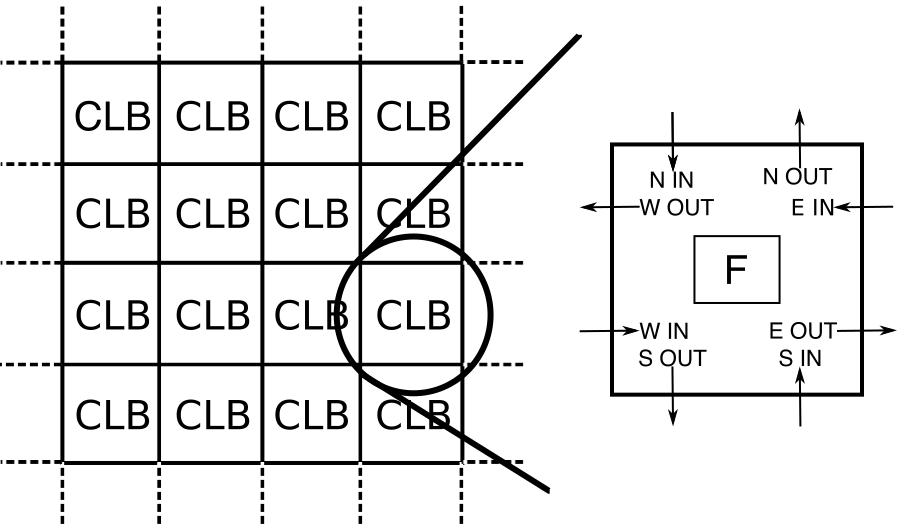
\includegraphics[width=.7\textwidth]{fpga.png}
\caption{FPGA architecture}
\label{fig:fpga}
\end{figure}

These immensly flexible circuits see wide use across industry. The most immediately
obvious example is
within firms developing more conventional integrated circuits who also ship accompanying
software. In these cases a team of engineers can develop software
while the hardware is developed in parallel, by using an FPGA loaded with a beta version
of chip. This avoids the many month wait times for a finished chip to be fabricated.
Recently FPGAs have seen a great deal of use as deep learning accelerators and cryptocurrency
miners; this is because FPGAs
configurations are cheaper to develop than ASIC hardware, are similarly highly application specific,
and see huge performance and power consumption benefits over more general purpose
hardware (GPGPUs for example). The flexibility also means iterative improvements
can be made to coincide with new discoveries without the need to purchase new
hardware. Similarly many industrial (and military) institutions require
bespoke hardware solutions to small-scale specific problems; maybe there is a
demand for a real time high performance
pump controller which will only be used in a handful of locations. In these situations,
more often than not, ASIC
development is too expensive and not worth the narrow application setting. This demand has resulted in
the widespread use of FPGAs
in roles requiring an ASIC but without the market pressure to drive the development
of one \cite{4267891}.
An application specific design can be built on an FPGA, while approaching peak performance and power
efficiency without massive development costs.
The military and aerospace sectors use FPGAs extensively for these reasons along with
the built-in cryptographic and anti-tamper hardware obfuscation capabilities of
military-grade FPGAs.

\todo ref all these use cases

\subsection{Genetic Algorithms}
The core of any genetic algorithm takes a randomly seeded population of binary strings
and applies
evolutionary pressure by performing a cycle of selection, crossover (an optional
step), and mutation
to move the population towards potential solutions to a given problem \cite{Goldberg:1989:GAS:534133}.
Beyond this there are many
variations, some of which will be explored in this thesis. The basic genetic algorithm is
outlined in Algorithm~\ref{alg:basic}.

\todo where does evaluatoin come itno this?

\begin{algorithm}[t]
	randomly initialise population $P$\;
	\While{evolving}{
		$P' \leftarrow Select( P )$\;
		$Crossover( P' )$\;
		$Mutate( P' )$\;
		$P \leftarrow P'$\;
	}
	\caption{Basic genetic algorithm}
	\label{alg:basic}
\end{algorithm}

\todo flesh out the algorithm (fitness function etc).

\todo first sentance in paragraph below is garbled

The binary string associated to an individual in the
population is considered the genotype, and a phenotype is what the string represents in the
context of the problem. In a biology a genotype is an organism's DNA, and a phenotype is
the organism itself, the expression of the DNA. In the context of genetic algorithms
the genotype is a binary string which is mapped onto a phenotype (in evolvable
hardware, often an FPGA configuration).
Selection ($Select$) generates a new population by evaluating each member of the
original population then
randomly choosing an individual from the old population based on a selection scheme,
the most common schemes will be outlined in Chapter~\ref{chap:technical}.
This selection step is repeated until the population is filled.
\todo crossover definition is wrong
Crossover ($Crossover$) randomly pairs each member of the new population
and given a probability swaps the genetic material from one individual with another from a
random selected point in the bitstring. Given an expected mutation-per-individual $m$, and
individual bitstring length
$l$ the $Mutate$ function iterates over each bit in each bitstring flipping the bit with
probability $\frac{m}{l}$. These simple processes coalesce into a high performance robust search
procedure.

\todo above section too fast, use diagrams to explain how each of them operates

\subsection{Genetic Algorithms with an FPGA Configuration}
Given a mapping from binary string to FPGA configuration and an FPGA test bed, one can
evaluate a population of bitstrings as the FPGA configuration to solve some digital
problem. This framework is at the core of evolutionary hardware. The bottleneck for physical evolvable
hardware is often the evaluation step, this involves converting each individual
to an FPGA configuration, uploading each in turn
to the FPGA and extensively testing it. When each upload takes in the order of
multiple seconds the evolution process can be laborious. To resolve this problem
many platforms simulate an FPGA until a design is chosen to be deployed, this reduces
training time aggressively, and is the direction this project has taken.

\todo talk about evolutionary dead ends

\section{Dynamic Problems}

\todo provide an example of a dynamic problem
A problem with evaluation critera which shifts over time is termed a dynamic problem. Designing
evolutionary hardware robust to this set of problems is of considerable benefit as
dynamic problems span a class of practical but notoriously problematic challenges including
real-time optimisation, and fault tolerance.

\subsection{Hardware Faults}
Hardware faults are catastrophic for electronic devices. A relatively short life span is
mostly accepted, and is relatively benign in many areas. But when the cost of replacement is
extraordinarily high or the scale of the operation is large enough there are huge benifits
to improving the fault tolerance of devices. An extreme example of the high cost of replacement
can be found with satellites, surveys of in-orbit satalites reveal that once deployed the
reliability of satalites drops aggressively, and despite the highest manufacturing standards
after 15 years reliability drops to below
90\% \cite{CASTET20091718}. Be it due micrometeor impacts,
or the ionising effects of radiation, satellites are known to fail and a great deal of
work is expended improving their reliability. With the cost
of putting a satellite into orbit set in the millions of pounds extending the lifespan
of such devices would have significant economic impact.

A little closer to home, data centres are vast structures contain thousands of servers.
Each of these has an 8\% probability of experiencing a failure each year
 \cite{Vishwanath:2010:CCC:1807128.1807161}.
Individually this is of no great concern, but when compounded across an entire data centre
server recovery and replacement becomes a primary concern for the management of
such an establishment.

One popular use of dynamic problems in evolutionary hardware is designed to breed
fault tolerance into a
design. This involves repeatedly turning on and off simulated faults in the FPGA during
evaluation in order to
create a design both robust to faults and dependent on faults, as could happen if
only evaluated in a faulty system \cite{651463}. Another fault resilience
technique requires evaluating the configuration
against a fault-free FPGA and then combining the result with evaluation runs on FPGAs
simulating known frequent faults \cite{651463}\cite{Keymeulen2000}. These faults could include component
wearout, and manifest as blocked communicatoins between CLBs or render the function
performed by a CLB innert. This extension of the fitness function (rather than
mid-execution fitness function modification) removes this approach from the domain of dynamic problems,
but it is worth noting as an alternate method to improve circuit reliability.

All of these methods require faults to be set before the genetic process begins, and can only be used to
develop evolveable hardware tolerant to specific faults. This requires a huge amount of knowledge
about the underlying hardware implementation and the frequency and severity of faults to generate
accurate fault models. This
is an important avenue of exploration but with evolvable hardware there is a missed
opportunity with a system capable of quick iterative improvements to work around
a problem as it occurs. This idea has been briefly explored in \cite{10.1007/3-540-61093-6_6}.

\todo explain why this is an important avenue of exploration

\subsection{Dynamic optimisation}
Another sucessful area of dynamic problems with evolutionary hardware involves
extending the evaluation function when a perfect solution has been found \cite{785435}. For example,
one could successfully evolve an audio filter and then incorporate a measure of "smallness"
into the fitness. This would add evolutionary pressure to not only be correct but also
use as little of the FPGA resources as possible.

Little work has been done exploring the reaction of evolvable hardware to tackling
related-but-not-identical problems (addition and subtraction, for example), and observing
the effect of varying
the relative benifits for correct answers of either on the performance of the circuit for each problem.
Information in this domain could
drive development of systems capable of dynamically optimising in real-time
under shifting conditions.

\todo give a realistic example

\section{Project Aims}

The broad aim of this project is to develop an improved evolvable hardware
platform capable of effectively addressing dynamic problems. More specifically:
\begin{itemize}
	\item Apply the genetic algorithm from \cite{10.1007/3-540-63173-9_61} to
		the binary arithmetic problem.
	\item Combine state of the art genetic algorithms to improve
		evolvable hardware performance for binary arithmetic.
	\item Explore the application of evolvable hardware to dynamic
		problems, including FPGA faults and weighted binary arithmetic.
	\item Develop a specialised FPGA simulator to act as the evaluation
		backend for the genetic algorithm.
	\item Study and improve the scaling performance of evolvable hardware.
\end{itemize}

\section{Project Challenges}
The project is not without challenges:
\begin{itemize}
	\item There are few ways to evaluate individuals and population health beyond how
		correct they are, so understanding why a system works or does not work may
		be difficult.
	\item The issue of scaling will slow development of anything other than
		trivial problems (2-bit addition and subtraction).
	\item FPGA configurations for a variety of problems investigated here are very fragile, in the
		context of evolution. Frequent mutations could be disastrous.
	\item More so than in many evolutionary contexts the prospect of evolutionary dead ends
		and dominating local optima will need to be addressed.
\end{itemize}
